\chapter{Исследовательская часть}

\section{Технические характеристики устройства}

Тестирование проводилось на устройстве со следующими техническими характеристиками:

\begin{itemize}
	\item операционная система Window 10 Home Single Language;
	\item память 8 Гб;
	\item процессор 11th Gen Intel(R) Core(TM) i7-1165G7 2.80 ГГц, 4 ядра.
\end{itemize}

\section{Демонстрация работы программы}
На рисунках \ref{fig:ex1} -- \ref{fig:ex2} приведены примеры работы программы поиска в двоичном дереве поиска несбалансированном и сбалансированном.
\begin{figure}[h]
	\centering
	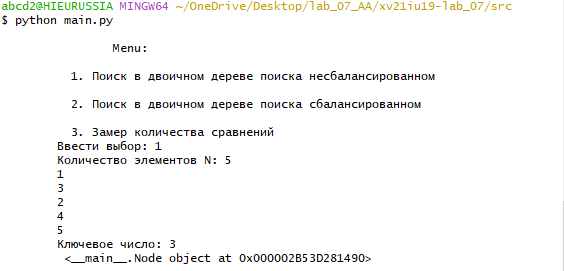
\includegraphics[scale=0.9]{img/ex1.png}
	\caption{Пример работы программы поиска в двоичном дереве поиска несбалансированном}
	\label{fig:ex1}
\end{figure}
\clearpage
\begin{figure}[h]
	\centering
	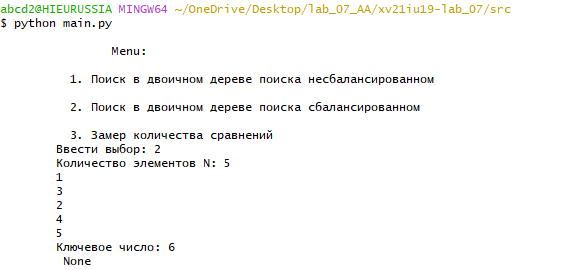
\includegraphics[scale=0.9]{img/ex2.png}
	\caption{Пример работы программы поиска в двоичном дереве поиска сбалансированном.}
	\label{fig:ex2}
\end{figure}

\section{Сравнение количество сравнений}

В ходе эксперимента было подсчитано количество сравнений, которые понадобились, чтобы найти каждый ключ в двоичном дереве поиска несбалансированном и сбалансированном, и на основе полученных данных составлены гистограммы.

Гистограммы для алгоритма поиска в двоичном дереве поиска несбалансированном в случае отсутствия элемента и случае нахождения элемента в листе на максимальной высоте дерева представлены на рисунке \ref{fig:bst2}

\begin{figure}[h]
	\centering
	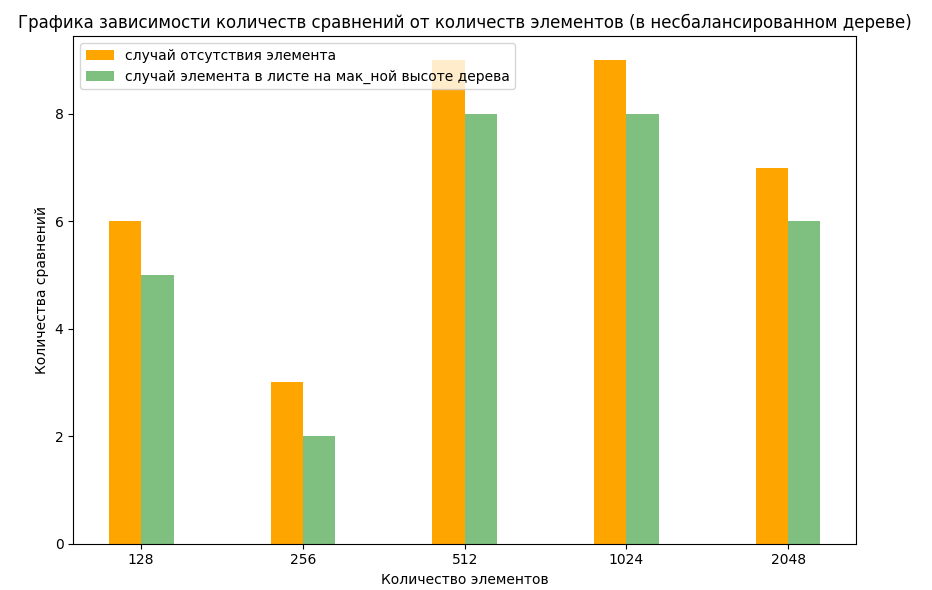
\includegraphics[scale=0.7]{img/exp_bst1.png}
	\caption{Сравнение количеств сравнений алгоритмов поиска в двоичном дереве поиска несбалансированном}
	\label{fig:bst2}
\end{figure}

Гистограммы для алгоритма поиска в двоичном дереве поиска сбалансированном в случае отсутствия элемента и случае нахождения элемента в листе на максимальной высоте дерева представлены на рисунке \ref{fig:avl}

\begin{figure}[h]
	\centering
	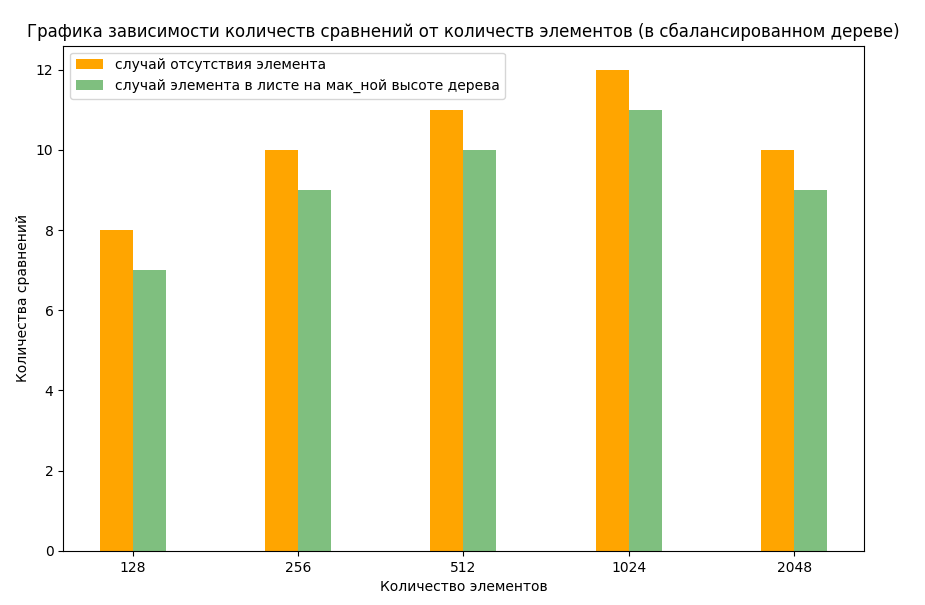
\includegraphics[scale=0.7]{img/exp_avl.png}
	\caption{Сравнение количеств сравнений алгоритмов поиска в двоичном дереве поиска сбалансированном}
	\label{fig:avl}
\end{figure}

\clearpage
\section{Вывод}

В результате замеров количеств сравнений алгоритмов поиска в случае отсутствия элемента или случае нахождения элемента в листе на максимальной высоте дерева было установлено, что случай отсуствия является худшим.



